\documentclass[14pt,a4paper]{extarticle}

% Компиляция: XeLaTeX или LuaLaTeX.
% Настройки под рекомендации по оформлению курсовых работ:
% A4, поля 25/15/25/20 мм, Times New Roman 14,
% абзацный отступ 12 мм, одинарный интервал, номер страницы справа сверху.

\usepackage{fontspec}
\usepackage{polyglossia}
\setmainlanguage{russian}
\setotherlanguage{english}

\setmainfont{Times New Roman}
\newfontfamily\cyrillicfont{Times New Roman}[Script=Cyrillic]
\newfontfamily\cyrillicfonttt{Courier New}[Script=Cyrillic]

\usepackage{geometry}
\geometry{
    a4paper,
    left=25mm,
    right=15mm,
    top=25mm,
    bottom=20mm
}

\usepackage{setspace}
\singlespacing

\usepackage{indentfirst}
\setlength{\parindent}{12mm}
\setlength{\parskip}{0pt}

\usepackage{amsmath,amssymb}
\usepackage{graphicx}
\usepackage{enumitem}
\usepackage{booktabs}
\usepackage{longtable}
\usepackage{array}
\usepackage{caption}
\usepackage{float}
\usepackage{hyperref}
\usepackage{titlesec}
\usepackage{tocloft}
\usepackage{fancyhdr}
\usepackage{ragged2e}

\hypersetup{
    colorlinks=false,
    pdfborder={0 0 0}
}

\sloppy

\pagestyle{fancy}
\fancyhf{}
\fancyhead[R]{\fontsize{12}{12}\selectfont\thepage}
\renewcommand{\headrulewidth}{0pt}

\fancypagestyle{plain}{%
  \fancyhf{}%
  \fancyhead[R]{\fontsize{12}{12}\selectfont\thepage}%
  \renewcommand{\headrulewidth}{0pt}%
}

\newcommand{\sectionbreak}{\clearpage}

\titleformat{\section}
  {\normalfont\bfseries\fontsize{14}{14}\selectfont}
  {\hspace*{12mm}\thesection}
  {1em}
  {}

\titleformat{\subsection}
  {\normalfont\bfseries\fontsize{14}{14}\selectfont}
  {\hspace*{12mm}\thesubsection}
  {1em}
  {}

\titleformat{name=\section,numberless}
  {\normalfont\bfseries\fontsize{14}{14}\selectfont\centering}
  {}
  {0pt}
  {}

\captionsetup[figure]{name={Рис.},labelsep=period,font=small,justification=centering}
\captionsetup[table]{name={Таблица},labelsep=period,font=small,justification=centering}

\begin{document}
\justifying

\thispagestyle{empty}
\begin{center}
Федеральное государственное автономное образовательное учреждение\\
высшего образования\\
«Национальный исследовательский университет\\
«Высшая школа экономики»\\[1em]

Факультет компьютерных наук\\[4em]

{\bfseries КУРСОВАЯ РАБОТА}\\[2em]

{\bfseries Классификация на архитектуре GraphSAGE на основе АФП}\\[0.5em]
{\bfseries Classification using GraphSAGE and FCA}\\[3em]

по направлению подготовки 01.04.02 Прикладная математика и информатика\\
образовательная программа «Науки о данных»
\end{center}

\vspace{5em}

\noindent\hfill
\begin{minipage}{8.5cm}
\normalfont\normalsize
\setlength{\parindent}{0pt}
\raggedright

Студент группы МНКДН251\\
Хайрисламов Тимур Айдарович

\vspace{1.8em}

Руководитель КР\\
Преподаватель, стажер-исследователь\\
Зуева Мария Михайловна

\end{minipage}

\vfill

\begin{center}
Москва, 2026
\end{center}

\clearpage

\setcounter{page}{2}
\renewcommand{\contentsname}{Содержание}
\tableofcontents
\clearpage

\section*{Введение}
\addcontentsline{toc}{section}{Введение}

Во многих прикладных задачах данные естественно задаются графом. Научные
публикации цитируют друг друга, пользователи взаимодействуют в социальных сетях,
белки образуют сети взаимодействий, а документы и веб-страницы соединяются
ссылками. В таких данных метка объекта зависит не только от его собственных
признаков, но и от окружения в графе. Поэтому для классификации узлов обычно
нужны методы, которые одновременно используют атрибутивную и структурную
информацию.

Одной из базовых архитектур такого типа является GraphSAGE. В отличие от ряда
трансдуктивных подходов, GraphSAGE обучает параметризованную функцию агрегации
соседских представлений, что делает его применимым к новым узлам и, в более
общем случае, к новым графам \cite{hamilton2017graphsage}. Эта особенность
особенно важна для задач классификации узлов в citation networks, где узлы
соответствуют научным публикациям, рёбра задают отношения цитирования, а
признаки узлов представляют текстовое содержание документов. На таких наборах
данных, как Cora, CiteSeer и PubMed, GraphSAGE, GCN и GAT стали стандартными
ориентирами для сравнения методов полунадзорной классификации узлов
\cite{yang2016planetoid,kipf2017gcn,velickovic2018gat}.

При этом результат GNN зависит не только от схемы message passing. Не менее
важно, какие признаки получает модель и как они были подготовлены. Упрощённые
feature-centric подходы, например SGC и SIGN, показывают, что заранее вычисленные
или сглаженные признаки иногда дают конкурентное качество даже при более простой
модели \cite{wu2019sgc,frasca2020sign}. Поэтому построение дополнительных
признаков для GraphSAGE в этой работе рассматривается как часть метода, а не как
нейтральный препроцессинг.

В настоящей работе рассматривается использование признаков, полученных из анализа
формальных понятий (АФП, Formal Concept Analysis, FCA). FCA представляет данные в
виде формального контекста: множества объектов, множества атрибутов и бинарного
отношения принадлежности объекта атрибуту. На основе этого контекста строятся
формальные понятия, каждое из которых задаётся объёмом объектов и содержанием
атрибутов \cite{ganter1999formal,wille1982restructuring}. С точки зрения
машинного обучения формальные понятия можно рассматривать как интерпретируемые
комбинации признаков. Если объект принадлежит объёму некоторого понятия, это
означает, что он обладает соответствующим набором атрибутов. Следовательно,
принадлежность объекта выбранным понятиям может быть использована как
дополнительное признаковое представление.

Интерес к такой постановке связан с более широкой линией работ, в которой FCA
используется не только как инструмент описательного анализа, но и как часть
моделей машинного обучения. В частности, в работах С.~О.~Кузнецова и соавторов
исследуется построение нейронных сетей на основе решёток формальных понятий
\cite{kuznetsov2017concept_lattice_nn}. В более современной работе
С.~О.~Кузнецова и М.~Зуевой предложена модернизация такой архитектуры,
FCA-CLNet, где предварительная кластеризация признаков используется для
построения более компактной и интерпретируемой нейросетевой модели
\cite{kuznetsov_zueva_training_nn_concepts}. Эта линия исследований показывает,
что формальные понятия могут выступать не только средством постфактум
интерпретации, но и конструктивным элементом архитектуры или признакового
пространства модели.

Другой важный аспект связан с отбором понятий. Полная решётка формальных понятий
может быть слишком большой для непосредственного использования, поэтому в
практических задачах необходимо выбирать ограниченное число наиболее полезных
понятий. В работе М.~Зуевой и С.~О.~Кузнецова исследуется влияние индексов
интересности формальных понятий на качество нейросетей, построенных на основе
концептных решёток. Рассматриваются, в частности, basic level, target entropy,
$\Delta$-stability и lift как критерии выбора понятий
\cite{zueva_kuznetsov_interestingness_nn}. Для настоящей работы это особенно
важно: мы также используем top-$K$ отбор понятий и проверяем, как критерии
выбора и способ построения формального контекста влияют на качество downstream
классификации.

Несмотря на близость этих исследований, наша постановка отличается от FCA-CLNet.
Мы не строим нейросетевую архитектуру непосредственно по решётке понятий и не
заменяем GraphSAGE FCA-моделью. Вместо этого формальные понятия используются как
дополнительные признаки узлов: для каждого выбранного понятия строится признак
принадлежности узла его объёму, после чего такие признаки конкатенируются с
исходными признаками и подаются на вход GraphSAGE. Тем самым работа проверяет
более узкий, но практически важный вопрос: могут ли concept-membership признаки
улучшить графовую нейронную сеть в задаче классификации узлов.

Ключевая методологическая трудность состоит в том, что улучшение качества после
добавления FCA-признаков не обязательно означает полезность именно
формально-понятийной структуры. Если к исходному признаковому описанию добавить
$K$ новых измерений, модель может выиграть просто из-за увеличения размерности
или дополнительной линейной проекции признаков. Поэтому в настоящей работе
FCA-признаки сравниваются не только с исходными признаками, но и с
размерностно-согласованным SVD-контролем. Такой контроль позволяет отделить
эффект добавленного признакового пространства от эффекта, связанного именно с
формальными понятиями.

Вторая трудность связана с концептуальным шкалированием. Классический FCA
работает с бинарным контекстом, тогда как признаки citation networks обычно
являются разреженными или взвешенными текстовыми векторами. Наивное шкалирование
\texttt{binary\_nonzero}, где любой ненулевой признак считается активным
атрибутом, может сводить понятия к одноатрибутным структурам. Тогда FCA-признаки
становятся похожи на обычный отбор отдельных признаков и почти не используют
связи между атрибутами. По этой причине conceptual scaling в работе вынесен в
отдельную экспериментальную ось: кроме наивного бинаризования рассматриваются
квантильное шкалирование и локальный top-$k$ отбор признаков. После основной
серии экспериментов эта линия была расширена до interval pattern structures:
вместо бинарной принадлежности к атрибутам проверяются интервальные описания
числовых признаков, soft membership и graph-aware построение интервалов.

Основной исследовательский вопрос работы формулируется следующим образом:
\textit{как способ описания объектов --- через бинарный формальный контекст или
через interval pattern structures --- влияет на полезность FCA-derived и
pattern-derived признаков для GraphSAGE в задаче классификации узлов?} Этот
вопрос объединяет две исследовательские линии: graph representation learning, где
важны качество входных признаков и графовая агрегация, и FCA-based learning, где
ключевую роль играют концептуальное шкалирование, отбор понятий,
membership-функции и интерпретируемость получаемых структур.

Цель работы --- исследовать применимость признаков, полученных из анализа
формальных понятий и interval pattern structures, в архитектуре GraphSAGE для
задачи классификации узлов на citation-network датасетах Cora, CiteSeer и
PubMed.

Для достижения цели решаются следующие задачи:
\begin{enumerate}[label=\arabic*)]
    \item реализовать воспроизводимый экспериментальный конвейер GraphSAGE + FCA
    для задачи классификации узлов;
    \item построить формальные контексты на основе признаков узлов и выделить
    формальные понятия;
    \item сформировать concept-membership и pattern-membership признаки и
    использовать их как дополнение к исходным признакам GraphSAGE;
    \item проверить hard и soft membership, а также graph-aware source для
    interval pattern structures;
    \item сравнить GraphSAGE на исходных признаках, GraphSAGE с FCA-признаками,
    GraphSAGE с pattern-derived признаками и GraphSAGE с SVD-контролем той же
    размерности;
    \item исследовать влияние концептуального шкалирования на структуру
    формального контекста, включая размеры intents/extents, покрытие узлов и долю
    многоатрибутных понятий;
    \item оценить, приводит ли более насыщенное шкалирование к улучшению качества
    классификации по сравнению с наивным FCA и SVD-контролем.
\end{enumerate}

Объектом исследования являются методы классификации узлов в графах. Предметом
исследования является влияние формально-понятийных и pattern-derived признаков,
а также способов концептуального шкалирования и membership, на качество
классификации в архитектуре GraphSAGE.

Основной вклад работы состоит в следующем. Реализован воспроизводимый
экспериментальный конвейер, в котором FCA-derived и pattern-derived признаки
добавляются к GraphSAGE и сравниваются с размерностно-согласованным SVD-контролем.
На структурной диагностике показано, что \texttt{binary\_nonzero} часто даёт почти
только одноатрибутные понятия. Затем проверены более насыщенные варианты
conceptual scaling, interval pattern structures, soft membership и graph-aware
source для построения patterns. Итоговый вывод остаётся условным: FCA-derived и
pattern-derived признаки не являются универсальным усилением GraphSAGE. Они дают
положительный результат на CiteSeer, graph-aware soft patterns оказываются
конкурентными на CiteSeer и PubMed, но Cora остаётся отрицательным случаем.
Следовательно, полезность таких признаков определяется не самим фактом добавления
понятий или patterns, а качеством описания объектов, способом задания membership
и критерием отбора признаков.

Работа организована следующим образом. В разделе 1 рассматриваются связанные
работы по графовым нейронным сетям, FCA, нейросетям на основе концептных решёток
и концептуальному шкалированию. В разделе 2 описывается методология исследования:
построение формального контекста, interval pattern structures, отбор понятий,
формирование дополнительных признаков, архитектура GraphSAGE и протокол оценки. В
разделе 3 приводятся экспериментальные результаты на Cora, CiteSeer и PubMed. В
разделе 4 обсуждаются полученные выводы, ограничения работы и возможные
направления дальнейшего исследования.

\section{Обзор связанных работ}

\subsection{Графовые нейронные сети и классификация узлов}

Задача классификации узлов является одной из базовых задач машинного обучения на
графах. В semi-supervised постановке метки доступны только для небольшой части
узлов, однако модель может использовать как признаки всех узлов, так и структуру
графа. Классические citation-network датасеты Cora, CiteSeer и PubMed получили
широкое распространение после работ по полунадзорному обучению на графах, в том
числе Planetoid \cite{yang2016planetoid}. На этих данных были проверены многие
архитектуры graph neural networks.

Одной из ключевых работ стала Graph Convolutional Network (GCN), где локальная
графовая структура используется через нормализованное распространение признаков
по соседям \cite{kipf2017gcn}. Позднее GraphSAGE предложил индуктивный механизм
агрегации соседей, допускающий обучение функции представления, применимой к
новым узлам \cite{hamilton2017graphsage}. GAT, в свою очередь, ввёл attention
механизм для взвешивания соседей \cite{velickovic2018gat}. Вместе эти работы
сформировали основу современной линии message passing neural networks.

Однако последующие исследования показали, что высокая эффективность GNN на
citation-сетях во многом зависит от преобразования признаков. SGC упрощает GCN
до предварительного сглаживания признаков и линейного классификатора, сохраняя
конкурентное качество \cite{wu2019sgc}. SIGN развивает эту идею, используя
заранее вычисленные многомасштабные признаки и избегая дорогого neighbor
sampling \cite{frasca2020sign}. Эти результаты важны для настоящей работы:
если сильные результаты могут быть получены за счёт преобразования признаков,
то любые дополнительные признаки, включая FCA-derived features, должны
сравниваться с сильными и честными признаковыми контролями.

\subsection{FCA в машинном обучении и интерпретируемости}

Formal Concept Analysis был предложен как математический аппарат для построения
иерархий понятий на основе бинарных отношений между объектами и атрибутами
\cite{wille1982restructuring,ganter1999formal}. В машинном обучении FCA
интересен тем, что формальные понятия задают одновременно группы объектов и
разделяемые ими наборы признаков. Такая двойственная структура делает FCA
естественным инструментом для интерпретируемого анализа данных, извлечения
правил, концептуальной кластеризации и feature construction.

Современные обзоры и tutorial-работы подчёркивают, что FCA полезен не только
как визуальный или логический аппарат, но и как источник интерпретируемых
структур для downstream-задач \cite{ignatov2017fca_tutorial,kwuida2021conceptml}.
При этом практическое использование FCA ограничено двумя факторами. Во-первых,
число формальных понятий может быть очень большим. Во-вторых, качество
полученных понятий существенно зависит от того, как построен формальный контекст.
Поэтому в прикладных задачах необходимы методы отбора понятий и меры
интересности. Работа С.~О.~Кузнецова и Т.~Махаловой по interestingness measures
формальных понятий показывает, что отбор понятий является центральной частью
применимой FCA-методологии, а не вспомогательной процедурой
\cite{kuznetsov2018interestingness}.

Эта линия особенно близка к настоящей работе, поскольку мы не используем всю
решётку понятий, а строим top-$K$ набор FCA-признаков. Следовательно, итоговое
качество зависит как от структуры формального контекста, так и от того, какие
понятия выбраны для передачи в GraphSAGE. В этом смысле работа находится на
стыке FCA-based feature construction и графового обучения.

\subsection{Нейронные сети на основе формальных понятий}

Связь FCA и нейросетевых моделей исследуется в ряде работ С.~О.~Кузнецова и
соавторов. В работе о neural network architecture based on concept lattices
предлагается строить архитектуру нейронной сети на основе концептной решётки
\cite{kuznetsov2017concept_lattice_nn}. В последующей работе С.~О.~Кузнецова и
М.~Зуевой предложена модернизация FCA-CLNet: признаки предварительно
кластеризуются в семантически интерпретируемые группы, затем на основе
полученного контекста выбираются устойчивые и интересные понятия, а по сокращённой
решётке строится компактная нейросетевая архитектура
\cite{kuznetsov_zueva_training_nn_concepts}. Такой подход ориентирован на
интерпретируемость и компактность модели при большом числе признаков.

Для настоящей работы эта линия важна по двум причинам. Во-первых, она показывает,
что формальные понятия можно использовать как конструктивный элемент обучения, а
не только как средство объяснения готовой модели. Во-вторых, она подчёркивает
важность предварительной обработки признаков, отбора понятий и сокращения решётки.
Наша работа развивает близкую идею в другой архитектурной среде: решётка понятий
не задаёт структуру нейросети напрямую, а выбранные понятия превращаются в
дополнительные признаки узлов для GraphSAGE.

Ещё более близкой к нашей экспериментальной логике является работа М.~Зуевой и
С.~О.~Кузнецова об индексах интересности для построения нейросетей на основе
концептных решёток \cite{zueva_kuznetsov_interestingness_nn}. В ней сравниваются
различные критерии выбора понятий, включая target entropy, lift и
$\Delta$-stability. Это напрямую мотивирует использование concept scorers и
top-$K$ selection в нашей работе. Различие состоит в том, что мы проверяем не
FCA-архитектуру как таковую, а добавленную ценность concept-membership признаков
в сильной графовой модели.

\subsection{Концептуальное шкалирование и числовые признаки}

Классический FCA работает с бинарными контекстами, но реальные данные часто
содержат числовые, взвешенные или категориальные признаки. Поэтому перед
построением формального контекста необходим этап концептуального шкалирования.
Для текстовых и citation-network данных это особенно существенно: признаки могут
быть разреженными bag-of-words индикаторами или взвешенными TF--IDF-подобными
величинами. Грубое преобразование ``ненулевой признак = активный атрибут''
теряет информацию о величине веса признака и может радикально изменить структуру
понятий.

В работах по numerical FCA подчёркивается, что переход от числовых признаков к
бинарному контексту не является нейтральным. Он может приводить к потере
информации, избыточному числу паттернов или, наоборот, к слишком грубым
одноатрибутным структурам \cite{kaytoue2011numericalfca}. Более общие подходы,
такие как pattern structures и scale-measures, развивают FCA для сложных
значений признаков и показывают, что выбор шкалирования должен рассматриваться
как содержательная часть метода \cite{gnedo1991patternstructures,hanika2021scalemeasures}.

Именно поэтому в настоящей работе conceptual scaling вынесен в отдельную
экспериментальную ось. Мы сравниваем наивное шкалирование
\texttt{binary\_nonzero} с более насыщенными схемами: \texttt{quantile\_global},
\texttt{topk\_per\_node} и \texttt{graph\_smoothed\_topk}. Это позволяет
проверить, является ли слабость FCA-признаков следствием самого подхода или
следствием неудачно построенного формального контекста.

\subsection{Размерностные контроли}

Если к исходному признаковому пространству добавить новые признаки, то улучшение
качества может возникнуть просто из-за увеличения размерности входа. Поэтому
сравнение FCA-признаков только с raw GraphSAGE недостаточно. Необходим контроль,
который добавляет такое же число признаков, но не использует формально-понятийную
структуру. В настоящей работе таким контролем является SVD: к исходным признакам
добавляется $K$-мерное низкоранговое представление той же ширины, что и набор
FCA-признаков.

Использование SVD-контроля согласуется с общей линией feature-centric GNN. Если
SVD той же размерности даёт качество, сопоставимое с FCA, то выигрыш нельзя
уверенно приписать именно понятиям. Напротив, если FCA превосходит SVD при
сопоставимой размерности, это является более сильным аргументом в пользу
содержательной роли концептуальных признаков. Такая постановка делает
экспериментальное сравнение более строгим и уменьшает риск переинтерпретации
результатов.

\section{Методология исследования}

\subsection{Постановка задачи}

В работе рассматривается задача классификации узлов в графе. Пусть задан граф
$G=(V,E)$, где $V$ --- множество узлов, $E$ --- множество рёбер. Каждому узлу
$v \in V$ соответствует вектор признаков $x_v \in \mathbb{R}^d$. Для части узлов
известны метки классов $y_v \in \{1,\ldots,C\}$. Необходимо построить модель,
которая по признакам узлов и структуре графа предсказывает метки тестовых узлов.

В citation-network датасетах узлы соответствуют научным публикациям, а рёбра ---
отношениям цитирования. Признаки узлов представляют текстовое содержание
документов. Все эксперименты проводятся в full-batch transductive постановке со
стандартным public-разбиением на train, validation и test. Общая схема
используемого конвейера показана на рис.~\ref{fig:model_diagram}: исходные
признаки узлов проходят через блок построения FCA-derived или pattern-derived
признаков, затем объединяются с исходным представлением и подаются в GraphSAGE.

\begin{figure}[H]
\centering
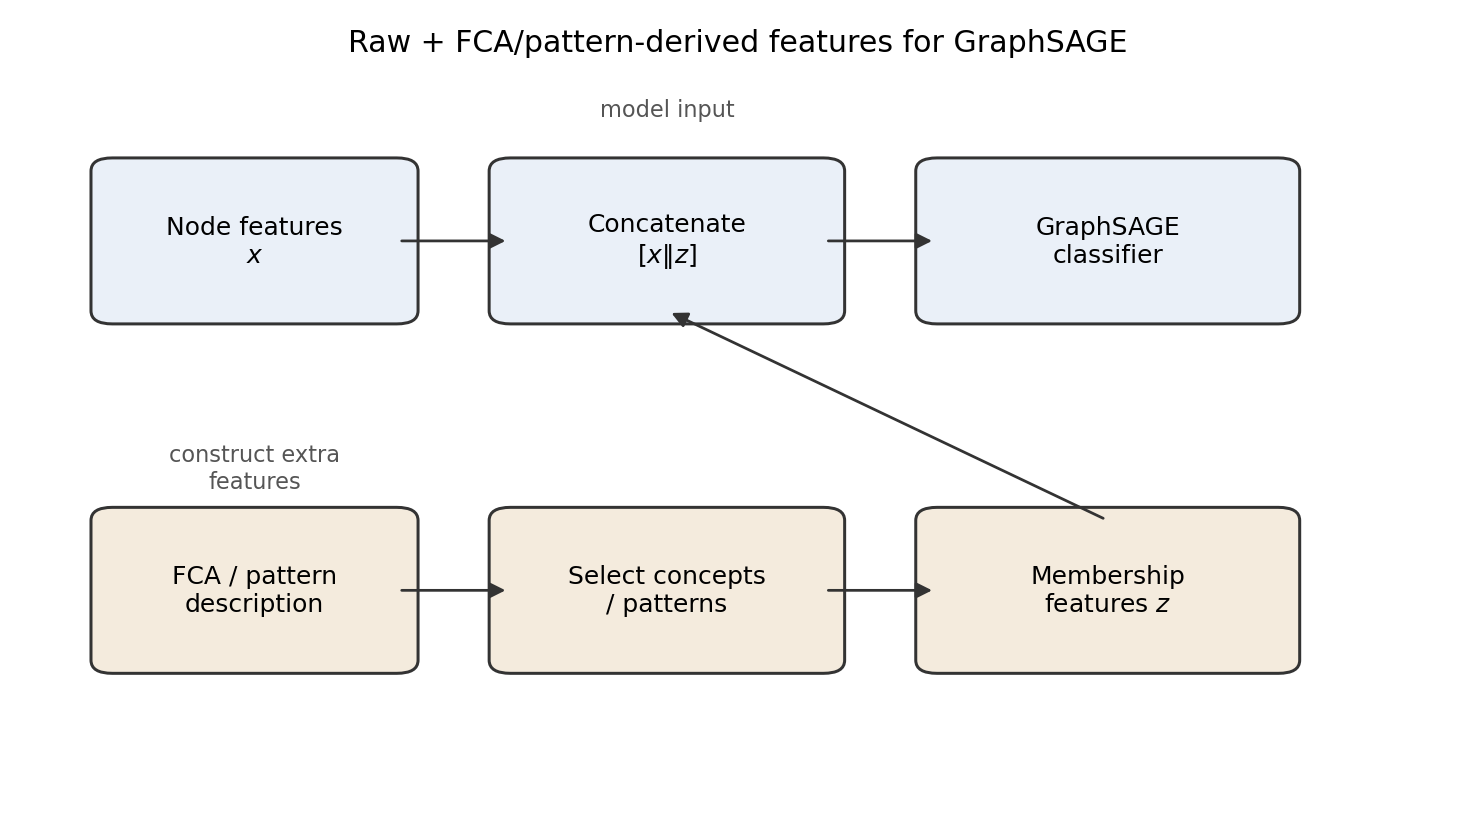
\includegraphics[width=\textwidth]{figures/model_diagram.png}
\caption{Схема объединения исходных признаков, FCA-derived / pattern-derived признаков и GraphSAGE}
\label{fig:model_diagram}
\end{figure}

\subsection{GraphSAGE}

В качестве основной графовой архитектуры используется двухслойный GraphSAGE с
mean aggregation. На каждом слое представление узла обновляется на основе его
текущего состояния и агрегированного представления соседей. Агрегация и
обновление задаются формулами~(\ref{eq:sage_agg}) и~(\ref{eq:sage_update}):
\begin{equation}
    h_{\mathcal{N}(v)}^{(k)} =
    \operatorname{mean}
    \left(
        \{h_u^{(k-1)}: u \in \mathcal{N}(v)\}
    \right),
    \label{eq:sage_agg}
\end{equation}
\begin{equation}
    h_v^{(k)} =
    \sigma
    \left(
        W^{(k)}
        \cdot
        \left[
            h_v^{(k-1)} \, \Vert \,
            h_{\mathcal{N}(v)}^{(k)}
        \right]
    \right),
    \label{eq:sage_update}
\end{equation}
где $\mathcal{N}(v)$ --- множество соседей узла, $\Vert$ обозначает
конкатенацию, $W^{(k)}$ --- обучаемая матрица, $\sigma$ --- нелинейность.

В экспериментах используется конфигурация: два слоя, 128 скрытых признаков,
dropout 0.5, Adam с learning rate 0.005 и weight decay $5\cdot 10^{-4}$.
Обучение проводится до 300 эпох с early stopping по validation accuracy.

\subsection{Построение формального контекста}

Для применения FCA исходные признаки узлов преобразуются в бинарный формальный
контекст, заданный формулой~(\ref{eq:formal_context}):
\begin{equation}
    \mathbb{K} = (G, M, I),
    \label{eq:formal_context}
\end{equation}
где $G$ --- множество объектов, в данной работе узлов графа; $M$ --- множество
атрибутов; $I \subseteq G \times M$ --- бинарное отношение принадлежности
объекта атрибуту.

Для подмножества объектов $A \subseteq G$ и подмножества атрибутов
$B \subseteq M$ операторы Галуа определяются формулами~(\ref{eq:galois_objects})
и~(\ref{eq:galois_attributes}):
\begin{equation}
    A' = \{m \in M \mid \forall g \in A: (g,m) \in I\},
    \label{eq:galois_objects}
\end{equation}
\begin{equation}
    B' = \{g \in G \mid \forall m \in B: (g,m) \in I\}.
    \label{eq:galois_attributes}
\end{equation}
Формальным понятием называется пара $(A,B)$ такая, что $A'=B$ и $B'=A$.
Множество $A$ называется объёмом понятия, а множество $B$ --- содержанием.

\subsection{Концептуальное шкалирование}

В работе сравниваются несколько способов построения бинарного контекста. Базовый
вариант \texttt{binary\_nonzero} задаёт атрибут как активный, если
соответствующее значение признака не равно нулю, как показано в
формуле~(\ref{eq:binary_nonzero}):
\begin{equation}
    I(g,m_j) = 1[x_{gj} \neq 0].
    \label{eq:binary_nonzero}
\end{equation}

В режиме \texttt{quantile\_global} для каждого признака вычисляется порог по
квантилю $q$ на обучающих узлах, после чего атрибут активируется по
формуле~(\ref{eq:quantile_global}), если значение признака не ниже этого порога:
\begin{equation}
    I(g,m_j) = 1[x_{gj} \geq Q_j(q)].
    \label{eq:quantile_global}
\end{equation}
В экспериментах используются $q=0.90$ для Cora и CiteSeer и $q=0.75$ для PubMed.

В режиме \texttt{topk\_per\_node} для каждого узла активируются только $k$
наибольших положительных признаков. Такой способ уменьшает число активных
атрибутов на объект и делает контекст более разреженным. Наконец,
\texttt{graph\_smoothed\_topk} сначала сглаживает признаки по соседям графа по
формуле~(\ref{eq:graph_smooth}):
\begin{equation}
    X_{\text{smooth}} = \alpha X + (1-\alpha)\hat{A}X,
    \label{eq:graph_smooth}
\end{equation}
где $\hat{A}$ --- нормализованная матрица смежности, после чего применяется
top-$k$ шкалирование.

\subsection{Pattern structures}

Бинарный формальный контекст удобен для классического FCA, но он неизбежно
теряет часть информации о числовых признаках. Поэтому дополнительно была
проверена более общая постановка на основе pattern structures
\cite{gnedo1991patternstructures}. В ней объекту сопоставляется не множество
бинарных атрибутов, а более сложное описание. В работе используется
interval-pattern вариант: описание задаётся набором признаков и интервалами
допустимых значений для каждого из них.

Пусть для выбранного pattern $P_j$ заданы признаки $F_j$ и интервалы
$[l_{jf}, u_{jf}]$ для каждого $f \in F_j$. Узел принадлежит extent такого pattern,
если его значения попадают во все соответствующие интервалы:
\begin{equation}
    z_{vj}^{\mathrm{pat}} =
    \mathbb{I}
    \left(
        \forall f \in F_j:
        l_{jf} \leq x_{vf} \leq u_{jf}
    \right).
    \label{eq:pattern_membership}
\end{equation}
Интервалы строятся по квантильным бинам, вычисленным на обучающих узлах. Кандидаты
pattern structures генерируются из выборки объектов: для каждого объекта берутся
несколько наиболее активных признаков, после чего соответствующие значения
заменяются интервалами квантильной сетки. Затем pattern structures фильтруются по
support, ранжируются теми же критериями support или target entropy и превращаются
в дополнительные признаки по формуле~(\ref{eq:pattern_membership}). Помимо hard
membership проверяется soft membership: вместо бинарного попадания в интервал
используется степень близости значения к центру интервала. Также рассматривается
graph-aware вариант, где интервалы строятся не по исходным признакам, а по смеси
исходных и сглаженных по соседям признаков. Этот вариант проверяет, помогает ли
более общее числовое описание объектов там, где бинарный FCA оказывается слишком
грубым.

\subsection{Отбор понятий и FCA-признаки}

После построения контекста извлекаются формальные понятия, затем они ранжируются
по функции оценки. В работе используются несупервизорный критерий support и
супервизорный критерий target entropy. Супервизорные оценки вычисляются только
по обучающим узлам, чтобы исключить утечку информации из тестовой выборки.

Из выбранных $K$ понятий строится матрица принадлежности узлов понятиям
(формула~(\ref{eq:fca_features})):
\begin{equation}
    z_v =
    \left[
        \mathbb{I}(v \in \operatorname{Ext}(C_1)),
        \ldots,
        \mathbb{I}(v \in \operatorname{Ext}(C_K))
    \right].
    \label{eq:fca_features}
\end{equation}
Итоговый вход модели задаётся конкатенацией исходных признаков и FCA-признаков
согласно формуле~(\ref{eq:concat_features}):
\begin{equation}
    \tilde{x}_v = x_v \Vert z_v.
    \label{eq:concat_features}
\end{equation}

\subsection{SVD-контроль и протокол оценки}

Для контроля эффекта добавленной размерности используется SVD-представление
исходных признаков той же ширины $K$. Низкоранговые представления такого типа
широко применяются в анализе текстовых признаков, включая latent semantic
analysis \cite{deerwester1990lsa}. В этом варианте на вход GraphSAGE подаётся
конкатенация исходных признаков и $K$ SVD-компонент. Такой контроль позволяет
проверить, превосходят ли FCA-признаки простое низкоранговое расширение
признакового пространства.

Все результаты усредняются по пяти random seeds: 0, 1, 2, 3, 4. Основные метрики
--- test accuracy и macro-F1. Дополнительно анализируется accuracy на узлах
малой степени, но эта метрика используется только как вспомогательная.
Конфигурация считается успешной, если она превосходит K-matched SVD более чем на
0.002 accuracy; если она превосходит только \texttt{binary\_nonzero} FCA, но не
SVD, результат считается частичным.

\subsection{Воспроизводимость экспериментов}

Эксперименты организованы как конфигурационный конвейер: параметры датасетов,
моделей, шкалирования и сеток перебора вынесены в YAML-файлы, а итоговые таблицы
строятся из per-seed результатов. Код экспериментов и файлы конфигурации доступны
в репозитории: \url{https://github.com/agiccoder/graphsage-fca-coursework}. Для
финальных сравнений используются только зафиксированные запуски по seeds 0--4 и
public-разбиения Cora, CiteSeer и PubMed. При построении таблиц richer scaling
отделяется от \texttt{binary\_nonzero} по режиму бинаризации и его параметрам, а
SVD-сравнение проводится при том же числе добавленных признаков $K$. Такая схема
нужна, чтобы не смешивать разные варианты шкалирования и не завышать эффект
FCA-признаков за счёт нестрогой агрегации.

\section{Экспериментальные результаты}

\subsection{Датасеты и базовые результаты}

В экспериментах используются три стандартных датасета: Cora, CiteSeer и PubMed.
Их основные характеристики приведены в табл.~\ref{tab:datasets}.

\begin{table}[H]
\centering
\caption{Характеристики используемых датасетов}
\label{tab:datasets}
\begin{tabular}{lrrrrrrr}
\toprule
Датасет & Узлы & Рёбра & Признаки & Классы & Train & Val & Test \\
\midrule
Cora & 2708 & 10556 & 1433 & 7 & 140 & 500 & 1000 \\
CiteSeer & 3327 & 9104 & 3703 & 6 & 120 & 500 & 1000 \\
PubMed & 19717 & 88648 & 500 & 3 & 60 & 500 & 1000 \\
\bottomrule
\end{tabular}
\end{table}

Сначала сравнивались raw GraphSAGE, MLP, GCN, наивный вариант
GraphSAGE + FCA при \texttt{binary\_nonzero} и SVD-контроль той же размерности
$K=128$. Результаты приведены в табл.~\ref{tab:main_results}.

\begin{table}[H]
\centering
\caption{Основные результаты при $K=128$}
\label{tab:main_results}
\begin{tabular}{llrrr}
\toprule
Датасет & Вариант & Accuracy & Macro-F1 & Low-degree acc. \\
\midrule
Cora & GraphSAGE raw & 0.8008 & 0.7929 & 0.7535 \\
Cora & FCA binary, support & 0.8010 & 0.7958 & 0.7525 \\
Cora & SVD control & 0.8116 & 0.8062 & 0.7605 \\
\midrule
CiteSeer & GraphSAGE raw & 0.6832 & 0.6426 & 0.6121 \\
CiteSeer & FCA binary, support & 0.6924 & 0.6585 & 0.6222 \\
CiteSeer & SVD control & 0.6924 & 0.6569 & 0.6158 \\
\midrule
PubMed & GraphSAGE raw & 0.7658 & 0.7613 & 0.7561 \\
PubMed & FCA binary, support & 0.6784 & 0.6911 & 0.6506 \\
PubMed & SVD control & 0.7616 & 0.7560 & 0.7510 \\
\bottomrule
\end{tabular}
\end{table}

Наивный FCA-вариант показывает неоднородные результаты. На CiteSeer он улучшает
raw GraphSAGE и достигает уровня SVD-контроля. На Cora результат близок к raw
GraphSAGE, но уступает SVD. На PubMed наблюдается существенное ухудшение:
accuracy падает с 0.7658 до 0.6784. На рис.~\ref{fig:bar_accuracy} видно, что
даже в базовом сравнении SVD является сильным ориентиром для FCA-признаков. Это
указывает на то, что простое добавление FCA-признаков не является универсальным
улучшением.

\begin{figure}[H]
\centering
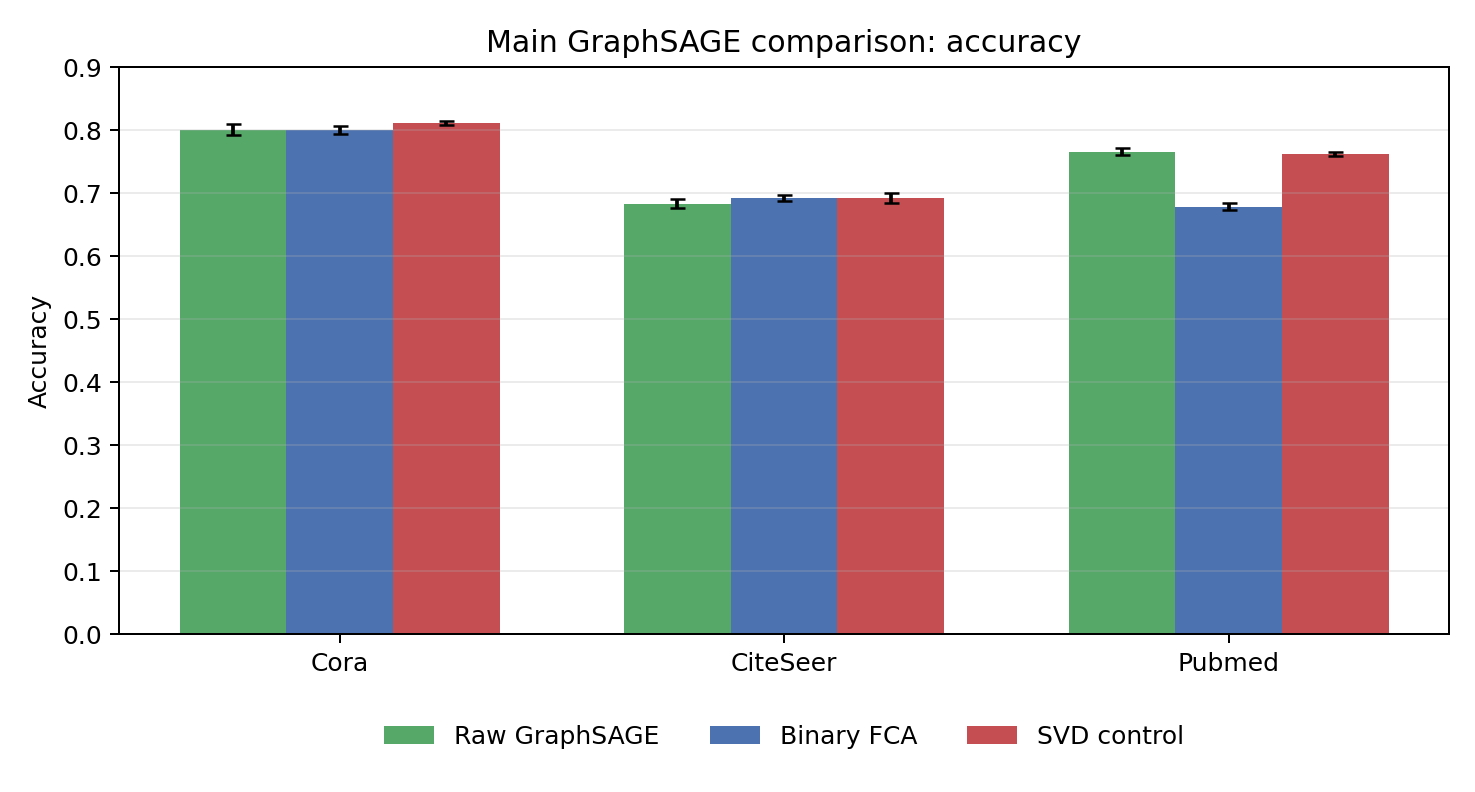
\includegraphics[width=0.85\textwidth]{figures/bar_accuracy.png}
\caption{Test accuracy для основных вариантов GraphSAGE, FCA и SVD-контроля}
\label{fig:bar_accuracy}
\end{figure}

\subsection{Структура формальных контекстов}

Для объяснения поведения FCA-признаков была проведена структурная диагностика
формальных контекстов. В табл.~\ref{tab:structural} сравниваются
\texttt{binary\_nonzero} и более насыщенные способы шкалирования.

\begin{table}[H]
\centering
\caption{Структурная диагностика формальных контекстов}
\label{tab:structural}
\begin{tabular}{llrrrr}
\toprule
Датасет & Шкалирование & Mean intent & Multi-attr & Coverage & Mean extent \\
\midrule
Cora & binary & 1.039 & 0.039 & 0.992 & 180.9 \\
Cora & quantile q=0.90 & 2.180 & 0.875 & 0.918 & 129.5 \\
CiteSeer & binary & 1.000 & 0.000 & 0.996 & 280.4 \\
CiteSeer & quantile q=0.90 & 1.773 & 0.688 & 0.988 & 188.5 \\
PubMed & binary & 1.000 & 0.000 & 1.000 & 3921.7 \\
PubMed & quantile q=0.75 & 2.211 & 0.742 & 0.999 & 1784.7 \\
PubMed & top-k, k=10 & 1.000 & 0.000 & 0.995 & 715.8 \\
\bottomrule
\end{tabular}
\end{table}

Из таблицы видно, что \texttt{binary\_nonzero} почти всегда приводит к
одноатрибутным понятиям: доля многоатрибутных понятий равна нулю на CiteSeer и
PubMed и составляет лишь 0.039 на Cora. Квантильное шкалирование, напротив,
создаёт более богатый контекст: доля многоатрибутных понятий достигает 0.688 на
CiteSeer и 0.742 на PubMed. Это подтверждает, что проблема наивного FCA связана
не только с GraphSAGE, но и с построением формального контекста.

\subsection{Richer scaling: влияние на качество классификации}

Далее проверялось, приводит ли более богатая структура контекста к улучшению
качества классификации. Основные результаты приведены в табл.~\ref{tab:richer}.

\begin{table}[H]
\centering
\caption{Результаты richer conceptual scaling}
\label{tab:richer}
\begin{tabular}{lllrrrr}
\toprule
Датасет & Scaling & Scorer & $K$ & FCA & SVD & $\Delta$ к SVD \\
\midrule
Cora & quantile q=0.90 & support & 128 & 0.7920 & 0.8116 & -0.0196 \\
Cora & quantile q=0.90 & target entropy & 128 & 0.7928 & 0.8116 & -0.0188 \\
\midrule
CiteSeer & quantile q=0.90 & support & 128 & 0.7028 & 0.6924 & 0.0104 \\
CiteSeer & quantile q=0.90 & target entropy & 128 & 0.6960 & 0.6924 & 0.0036 \\
CiteSeer & quantile q=0.90 & support & 256 & 0.7078 & 0.6870 & 0.0208 \\
CiteSeer & quantile q=0.90 & target entropy & 256 & 0.7108 & 0.6870 & 0.0238 \\
\midrule
PubMed & quantile q=0.75 & support & 128 & 0.7372 & 0.7616 & -0.0244 \\
PubMed & top-k, k=10 & support & 128 & 0.7510 & 0.7616 & -0.0106 \\
PubMed & graph-smoothed top-k & support & 128 & 0.7394 & 0.7616 & -0.0222 \\
\bottomrule
\end{tabular}
\end{table}

Самый убедительный положительный результат получен на CiteSeer. Квантильное
шкалирование при $q=0.90$ превосходит SVD-контроль той же размерности как при
$K=128$, так и при $K=256$. Лучший результат среди этих запусков достигается для
target entropy при $K=256$: accuracy равна 0.7108 против 0.6870 у
K-matched SVD-контроля и 0.6832 у raw GraphSAGE. При этом важно не смешивать два
сравнения: лучший SVD по всей сетке на CiteSeer немного выше (0.7116), поэтому
речь идёт именно о выигрыше над контролем при том же числе добавленных признаков.

На PubMed richer scaling существенно улучшает наивный FCA. Например,
\texttt{topk\_per\_node} при $K=128$ повышает accuracy с 0.6784 до 0.7510.
Однако этот результат всё ещё ниже raw GraphSAGE и SVD-контроля. Следовательно,
для PubMed richer scaling исправляет часть проблемы формального контекста, но
не делает FCA-признаки конкурентными с низкоранговым линейным представлением.

На Cora более насыщенное шкалирование не помогает. Лучший результат среди
FCA-вариантов для Cora достигается не richer scaling, а наивным
\texttt{binary\_nonzero} с target entropy: 0.8144, что практически соответствует
лучшему SVD-контролю, но не даёт устойчивого преимущества над ним.

\subsection{Эксперименты с pattern structures}

Отдельно была проведена проверка interval pattern structures. Цель этого
эксперимента состояла не в полной замене основного FCA-grid, а в проверке более
общего способа описания числовых признаков. Использовались квантильная сетка из
четырёх интервалов и patterns размера 2. После первоначального hard-варианта были
дополнительно проверены soft membership, graph-aware source, где pattern intervals
строятся по признакам, сглаженным по соседям графа, а также небольшой K-sweep для
$K \in \{64,128,256\}$. Основные результаты приведены в
табл.~\ref{tab:pattern_structures}.

\begin{table}[H]
\centering
\small
\caption{Ключевые результаты interval pattern structures}
\label{tab:pattern_structures}
\begin{tabular}{lllrrrrr}
\toprule
Датасет & Pattern-вариант & Scorer & $K$ & Pattern & SVD & $\Delta$ & 95\% CI \\
\midrule
Cora & graph-aware soft & target entropy & 128 & 0.8006 & 0.8116 & -0.0110 & [-0.0214; 0.0004] \\
CiteSeer & interval hard & support & 128 & 0.6800 & 0.6924 & -0.0124 & [-0.0230; -0.0150] \\
CiteSeer & interval soft & support & 128 & 0.6914 & 0.6924 & -0.0010 & [-0.0168; 0.0148] \\
CiteSeer & graph-aware soft & target entropy & 128 & 0.6988 & 0.6924 & 0.0064 & [-0.0038; 0.0178] \\
CiteSeer & graph-aware soft & target entropy & 256 & 0.6936 & 0.6870 & 0.0066 & [0.0008; 0.0124] \\
PubMed & interval hard & target entropy & 128 & 0.6890 & 0.7616 & -0.0726 & [-0.0710; -0.0710] \\
PubMed & interval soft & support & 128 & 0.7596 & 0.7616 & -0.0020 & [-0.0070; 0.0036] \\
PubMed & graph-aware soft & target entropy & 128 & 0.7672 & 0.7616 & 0.0056 & [0.0014; 0.0104] \\
PubMed & graph-aware soft & target entropy & 256 & 0.7794 & 0.7614 & 0.0180 & [0.0126; 0.0228] \\
\bottomrule
\end{tabular}
\end{table}
\normalsize

Результаты показывают, что простые hard interval patterns сами по себе не помогают:
на Cora, CiteSeer и PubMed они уступают SVD-контролю. Soft membership заметно
исправляет ситуацию, особенно на PubMed: interval soft повышает accuracy до
0.7596 и практически достигает SVD-контроля. Самый сильный вариант получается при
совмещении graph-aware source и soft membership. На CiteSeer положительный эффект
есть, но он небольшой: при $K=128$ доверительный интервал для разности с SVD
пересекает ноль, а при $K=256$ становится положительным. На PubMed эффект заметнее:
graph-aware soft pattern variant при $K=256$ достигает accuracy 0.7794 против
0.7614 у K-matched SVD и 0.7658 у raw GraphSAGE. Значит, pattern structures
сработали не в базовом hard-варианте, а после добавления мягкой принадлежности,
учёта графового окружения и настройки числа pattern-derived признаков. На
рис.~\ref{fig:pattern_delta_svd} отдельно показано, как основные pattern-варианты
при $K=128$ отличаются от K-matched SVD.

\begin{figure}[H]
\centering
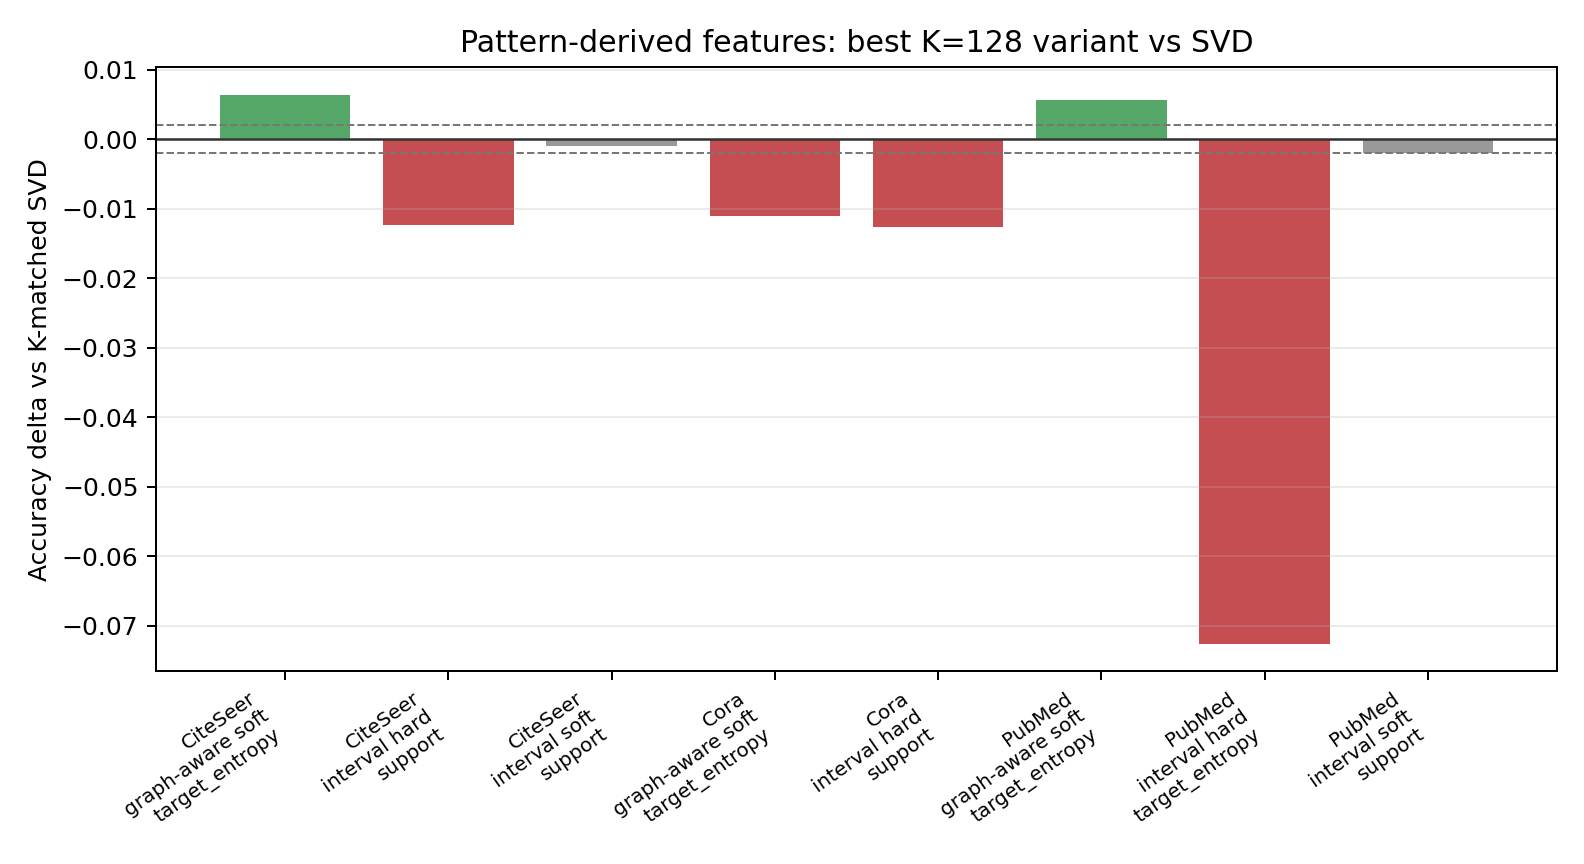
\includegraphics[width=0.9\textwidth]{figures/pattern_delta_vs_svd.png}
\caption{Разность accuracy между pattern-derived признаками и K-matched SVD при $K=128$}
\label{fig:pattern_delta_svd}
\end{figure}

\subsection{Лучшие FCA-конфигурации и роль pattern structures}

В табл.~\ref{tab:best_configs} приведены лучшие FCA-конфигурации для каждого
датасета.

\begin{table}[H]
\centering
\caption{Лучшие FCA-конфигурации по датасетам}
\label{tab:best_configs}
\begin{tabular}{llrrr}
\toprule
Датасет & Лучшая FCA-конфигурация & FCA & Raw & Best SVD \\
\midrule
Cora & binary, target entropy, $K=128$ & 0.8144 & 0.8008 & 0.8120 \\
CiteSeer & quantile q=0.90, target entropy, $K=256$ & 0.7108 & 0.6832 & 0.7116 \\
PubMed & top-k, support, $K=128$ & 0.7510 & 0.7658 & 0.7658 \\
\bottomrule
\end{tabular}
\end{table}

Таблица~\ref{tab:best_configs} учитывает только FCA-конфигурации, построенные
через бинарный формальный контекст и richer conceptual scaling. Если дополнительно
учитывать pattern-derived признаки, то для PubMed лучшим результатом становится
graph-aware soft pattern variant при $K=256$ с accuracy 0.7794, что выше raw
GraphSAGE и K-matched SVD. Этот результат рассматривается как отдельная
pattern-derived ветка, поскольку табл.~\ref{tab:best_configs} относится только к
FCA-конфигурациям.

Эти результаты не поддерживают простой тезис «FCA улучшает GraphSAGE». Эффект
зависит от датасета, шкалирования и отбора понятий. На CiteSeer richer scaling
выигрывает у SVD при фиксированном $K$, хотя лучший SVD по сетке остаётся
практически на том же уровне. На PubMed более богатое шкалирование улучшает
только FCA-семейство относительно наивного контекста. На Cora оно не даёт
прироста качества. На рис.~\ref{fig:scaling_delta_svd} показана только FCA-ветка
экспериментов, то есть результаты richer conceptual scaling без interval pattern
structures. Поэтому PubMed на рисунке остаётся ниже SVD, хотя graph-aware soft
patterns в табл.~\ref{tab:pattern_structures} дают другой результат.

\begin{figure}[H]
\centering
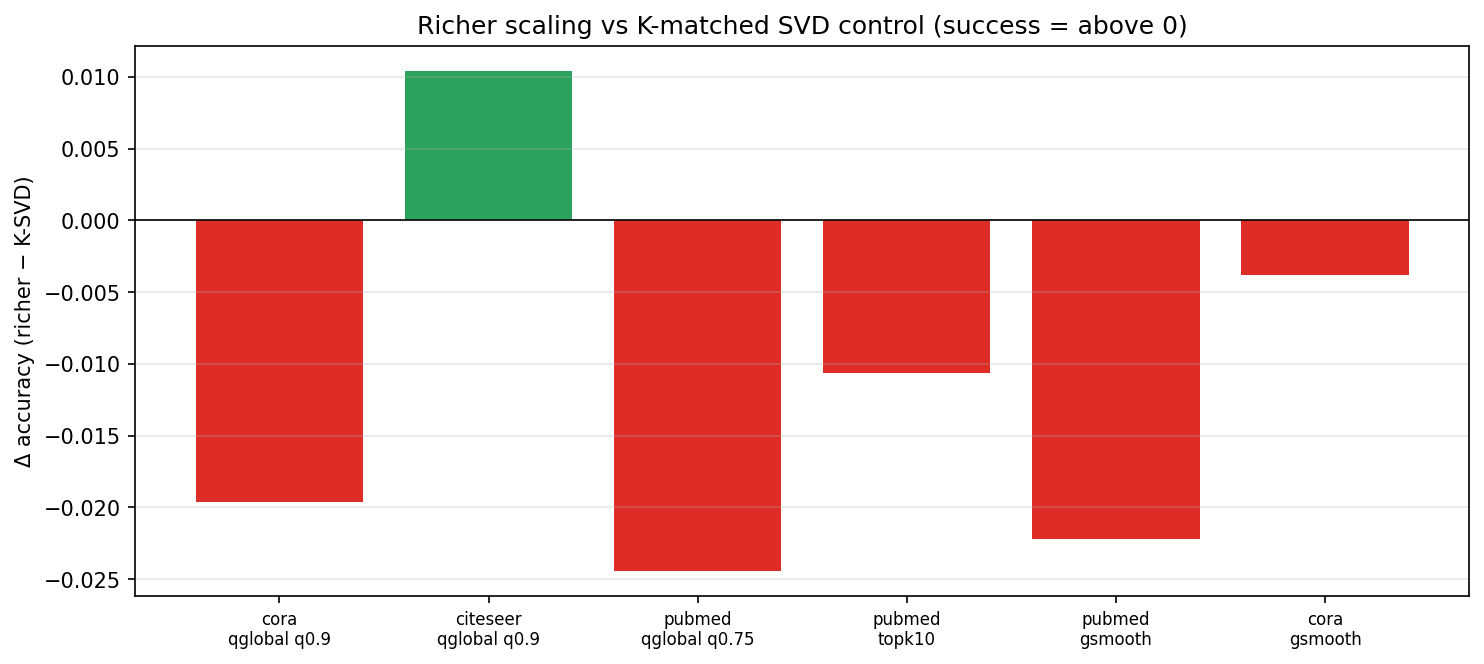
\includegraphics[width=0.85\textwidth]{figures/scaling_delta_vs_svd.png}
\caption{Разность accuracy между richer FCA и SVD-контролем без pattern structures}
\label{fig:scaling_delta_svd}
\end{figure}

\section{Обсуждение}

Эксперименты показывают, что FCA-признаки ведут себя по-разному на разных
датасетах. Они не работают как готовая добавка, которая автоматически усиливает
GraphSAGE: простое добавление признаков принадлежности формальным понятиям иногда
почти ничего не меняет, а иногда заметно ухудшает результат. На PubMed это видно
особенно хорошо: \texttt{binary\_nonzero} FCA сильно уступает raw GraphSAGE.
Такие отрицательные случаи важны для работы, потому что они не дают свести
результат к простой мысли «добавили признаков --- стало лучше».

Причина не сводится к самой архитектуре GraphSAGE. Структурная диагностика
показывает, что наивное бинаризование почти полностью сводит понятия к
одноатрибутным структурам. В таком виде FCA-признаки становятся близки к отбору
отдельных исходных признаков и теряют то, ради чего вообще используется FCA:
описание групп объектов через совместные наборы атрибутов. Квантильное
шкалирование исправляет структуру контекста: появляются многоатрибутные понятия,
а extents становятся меньше. Но это ещё не гарантирует рост accuracy. Проверка
pattern structures уточняет этот вывод: hard interval descriptions также не
достаточны, зато soft membership и graph-aware построение интервалов помогают на
CiteSeer и особенно на PubMed.

Именно поэтому в работе нужен SVD-контроль. Если сравнивать только с raw
GraphSAGE или с наивным FCA, вклад формальных понятий легко переоценить.
K-matched SVD показывает, какая часть эффекта может быть связана просто с
добавлением новых измерений. По этой более строгой проверке для классических
FCA-признаков положительный результат остаётся прежде всего на CiteSeer: richer
FCA превосходит SVD при одинаковом $K$. На Cora и PubMed такие FCA-признаки не
превосходят SVD. Однако interval pattern structures образуют отдельный
exploratory case: graph-aware soft patterns оказываются конкурентными с SVD на
CiteSeer и превосходят SVD на PubMed при $K=256$.

По отношению к FCA-CLNet эта работа занимает более осторожную позицию. В
FCA-CLNet формальные понятия задают структуру нейросети, а здесь они используются
как дополнительные признаки для уже существующей графовой модели. Такой вариант
архитектурно проще, зато позволяет отдельно проверить добавленную ценность
concept-membership признаков. Результаты говорят не о том, что FCA всегда полезен
для GNN, а о том, что он может быть полезен при удачном шкалировании и подходящем
датасете. Эксперимент с pattern structures показывает похожую границу. Само
интервальное описание ещё не решает проблему отбора полезных признаков для
GraphSAGE, но мягкая принадлежность и graph-aware построение интервалов делают
такие признаки конкурентными на CiteSeer и PubMed.

Возможное объяснение различий между датасетами состоит в балансе между
специфичностью понятий и покрытием узлов. На CiteSeer квантильное шкалирование
увеличивает долю многоатрибутных понятий при высоком покрытии. На Cora richer
scaling, судя по результатам, делает признаки менее полезными для классификатора,
а на PubMed даже улучшенные контексты остаются недостаточно конкурентными по
сравнению с raw и SVD-признаками. Это объяснение требует отдельной проверки и в
данной работе рассматривается как гипотеза, а не как доказанный причинный
механизм.

Работа имеет несколько ограничений. Во-первых, эксперименты проводились только
на трёх citation-network датасетах, поэтому выводы нельзя напрямую переносить на
другие типы графов. Во-вторых, использовалась относительно простая
GraphSAGE-архитектура, поскольку целью было изучить влияние признаков, а не
достичь максимального качества. В-третьих, интерпретация самих понятий
ограничена тем, что признаки Planetoid-датасетов не всегда имеют легко
восстанавливаемые семантические имена. Отдельным ограничением является малое
число random seeds. В работе сравниваются средние значения по пяти запускам, но
не проводится формальная проверка статистической значимости различий. Поэтому
небольшие разрывы между конфигурациями, особенно на Cora и CiteSeer, следует
интерпретировать осторожно. Эксперимент с pattern structures также ограничен:
использовались фиксированный размер pattern и фиксированная квантильная сетка, а
K-sweep был проведён только для CiteSeer и PubMed. Наконец, хотя richer scaling и
graph-aware soft patterns дают более сильные признаки, остаётся открытым вопрос о
более сложных pattern structures и устойчивых понятиях, которые могут оказаться
более информативными.

Дальше эту линию стоит развивать не как простой переход к pattern structures ---
он уже сделан в базовом interval-варианте, --- а как поиск более удачных pattern
описаний и критериев отбора. В первую очередь интересны меры устойчивости,
включая $\Delta$-stability \cite{buzmakov2015patternstructures}, интервалы
переменной ширины, graph-aware отбор patterns и проверка на гетерофильных графах.
Отдельно полезны датасеты, где признаки имеют понятную семантику: на них можно
оценивать не только accuracy, но и содержательность найденных понятий.

\section*{Заключение}
\addcontentsline{toc}{section}{Заключение}

В работе исследована возможность использовать признаки, полученные из анализа
формальных понятий и interval pattern structures, для улучшения GraphSAGE в задаче
классификации узлов. Построен экспериментальный конвейер, в котором из признаков
узлов формируется бинарный формальный контекст или интервальное описание объекта,
после чего выбранные concept-membership и pattern-membership признаки добавляются
к исходному представлению узла.

Полученные результаты показывают, что FCA-derived и pattern-derived признаки не
являются универсальным усилением GraphSAGE. Для классического бинарного FCA
устойчивый положительный результат наблюдается прежде всего на CiteSeer. Однако
проверка interval pattern structures показывает, что более гибкое числовое
описание объектов, особенно в сочетании с soft membership и graph-aware source,
может быть конкурентным с SVD-контролем на CiteSeer и превосходить его на PubMed
при $K=256$. Поэтому главный фактор успеха состоит не в самом факте использования
FCA, а в качестве описания объектов, способе задания membership и критерии отбора
признаков.

В дальнейшем эту линию стоит развивать через более аккуратный отбор устойчивых
понятий и patterns, интервалы переменной ширины и расширенные graph-aware
варианты шкалирования. Отдельно полезна проверка на датасетах с более понятной
семантикой признаков: там можно оценивать не только accuracy, но и содержательную
интерпретируемость найденных понятий.

\renewcommand{\refname}{Список использованных источников}
\addcontentsline{toc}{section}{Список использованных источников}

\begin{thebibliography}{99}

\bibitem{wille1982restructuring}
Wille R. Restructuring lattice theory: An approach based on hierarchies of concepts //
Ordered Sets. Dordrecht: Springer, 1982. P. 445--470.

\bibitem{ganter1999formal}
Ganter B., Wille R. Formal Concept Analysis: Mathematical Foundations.
Berlin: Springer, 1999.

\bibitem{yang2016planetoid}
Yang Z., Cohen W. W., Salakhutdinov R.
Revisiting Semi-Supervised Learning with Graph Embeddings //
International Conference on Machine Learning. 2016. P. 40--48.

\bibitem{kipf2017gcn}
Kipf T. N., Welling M.
Semi-Supervised Classification with Graph Convolutional Networks //
International Conference on Learning Representations. 2017.

\bibitem{hamilton2017graphsage}
Hamilton W. L., Ying R., Leskovec J.
Inductive Representation Learning on Large Graphs //
Advances in Neural Information Processing Systems. 2017.

\bibitem{velickovic2018gat}
Veličković P., Cucurull G., Casanova A., Romero A., Liò P., Bengio Y.
Graph Attention Networks //
International Conference on Learning Representations. 2018.

\bibitem{wu2019sgc}
Wu F., Zhang T., Souza A. H., Fifty C., Yu T., Weinberger K. Q.
Simplifying Graph Convolutional Networks //
International Conference on Machine Learning. 2019. P. 6861--6871.

\bibitem{frasca2020sign}
Frasca F., Rossi E., Eynard D., Chamberlain B., Bronstein M., Monti F.
SIGN: Scalable Inception Graph Neural Networks //
ICML Workshop on Graph Representation Learning and Beyond. 2020.

\bibitem{ignatov2017fca_tutorial}
Ignatov D. I.
Introduction to Formal Concept Analysis and Its Applications in Information Retrieval and Related Fields //
Russian Summer School in Information Retrieval. 2017.

\bibitem{kwuida2021conceptml}
Kwuida L., Sertkaya B.
Formal Concept Analysis in Machine Learning and Knowledge Discovery //
Concept Lattices and Their Applications. 2021.

\bibitem{kuznetsov2018interestingness}
Kuznetsov S. O., Makhalova T.
On interestingness measures of formal concepts //
Information Sciences. 2018. Vol. 442--443. P. 202--219.

\bibitem{kuznetsov2017concept_lattice_nn}
Kuznetsov S. O., Makhazhanov N., Ushakov M.
On Neural Network Architecture Based on Concept Lattices //
Foundations of Intelligent Systems: 23rd International Symposium, ISMIS 2017.
Springer, 2017. P. 653--663.

\bibitem{kuznetsov_zueva_training_nn_concepts}
Kuznetsov S. O., Zueva M.
Training Neural Networks Based on Formal Concepts //
FCA4AI@ECAI. 2024. P. 39--46.

\bibitem{zueva_kuznetsov_interestingness_nn}
Zueva M., Kuznetsov S. O.
Interestingness Indices for Building Neural Networks Based on Concept Lattices //
Automation and Remote Control. 2024. Vol. 85. No. 3. P. 297--304.

\bibitem{kaytoue2011numericalfca}
Kaytoue M., Kuznetsov S. O., Napoli A.
Revisiting Numerical Pattern Mining with Formal Concept Analysis //
Proceedings of the Twenty-Second International Joint Conference on Artificial Intelligence. 2011.

\bibitem{gnedo1991patternstructures}
Ganter B., Kuznetsov S. O.
Pattern Structures and Their Projections //
Conceptual Structures: Broadening the Base. Berlin: Springer, 2001.
P. 129--142.

\bibitem{buzmakov2015patternstructures}
Buzmakov A., Kuznetsov S. O., Napoli A.
Scalable Estimates of Concept Stability //
Formal Concept Analysis: 12th International Conference, ICFCA 2014.
Springer, 2014. P. 157--172.

\bibitem{hanika2021scalemeasures}
Hanika T., Hirth J.
Scale-measures for Formal Concept Analysis //
International Conference on Formal Concept Analysis. 2021.

\bibitem{deerwester1990lsa}
Deerwester S., Dumais S. T., Furnas G. W., Landauer T. K., Harshman R.
Indexing by latent semantic analysis //
Journal of the American Society for Information Science. 1990. Vol. 41, No. 6.
P. 391--407.

\end{thebibliography}

\end{document}
